%----------------------------------------------------------------------------------------
%	SECTION 1.1
%----------------------------------------------------------------------------------------

\section{The Fundamental Groupoid}

\begin{definition}
    Let $f:_ \xrightarrow{} X$ and $g:I \xrightarrow{} X$ be paths with
    $f(1)=g(0)$. We define \textbf{path multiplication} to be the operation
    \begin{equation*}
       f \ast g= \begin{cases}
                   f(2t), & \text{ if } 0 \leq t \leq \frac{1}{2}   \\
                   g(2t-1), & \text{ if } \frac{1}{2} \leq t \leq 1   \\
              \end{cases}
    \end{equation*}
    We call $f \ast g$ the  \textbf{path product} of $f$ and  $g$.
\end{definition}

\begin{lemma}\label{4.1.1}
    The path product of two paths is a continuous map.
\end{lemma}
\begin{proof}
    This follows from the pasting lemma.
\end{proof}
\begin{corollary}
    The path product is a path.
\end{corollary}
\begin{proof}
    Notice that if $f$ and  $g$ are paths with  $f(1)=g(0)$, then $f \ast
    g(0)=f(0)$ and $f \ast g(1)=g(1)$.
\end{proof}

\begin{definition}
    Let $X$ be a topological space and $A$ a subspace of $X$ Let $f_0:X
    \xrightarrow{} Y$ and $f_1:X \xrightarrow{} Y$, are continuous maps with
    $f_0|_A=f_1|_A$. we say that $f_0$ is \textbf{homotopic} to $f_1$
    \textbf{relative} $A$, and write $f_0 \simeq f_1 \rel{A}$ or $f_0 \simeq_A
    f_1$, if there is a continuous map $F:X \times I \xrightarrow{} Y$ that
    defines a homotpy between $f_0$ and $f_1$, and $F(a,t)=f_0(a)=f_1(a)$ for
    all $a \in A$. We call $F$ the \textbf{relative homotopy}.
\end{definition}

\begin{lemma}\label{4.1.2}
    Relative homotopy is an equivalence relation.
\end{lemma}

\begin{definition}
    Let $\partial{I}$ be the boundry of $I=[0,1]$ in $\R$. The equivalence class
    of  $f:I \xrightarrow{} X \rel{\partial{I}}$ is called the \textbf{path
    class} of $f$, and denoted $[f]$.
\end{definition}

\begin{theorem}\label{4.1.3}
    Let $f_0,f_1$ and $g_0,g_1$ be paths on $X$ with  $f_0 \simeq f_1
\rel{\partial{I}}$ and $g_0 \simeq g_1 \rel{\partial{I}}$. If $f_0(1)=g_0(0)$
and $f_1(1)-g_1(0)$ then $f_0 \ast g_0 \simeq f_1 \ast g_1 \rel{\partial{I}}$.
\end{theorem}
\begin{proof}
    Let $F:f_0 \sim_{\partial{I}} f_1$ and $G:g_0 \sim_{\partial{I}} g_1$ be the
    relative homotopies between $f_0$ and $f_1$, and $g_0$ and $g_1$,
    respectively. Define the map $H:I \times I \xrightarrow{} Y$ by
    \begin{equation*}
        H(s,t)=\begin{cases}
                F(2t,s), & \text{ if } 0 \leq t \leq \frac{1}{2}    \\
                G(2t-1,s), &, \text{ if } \frac{1}{2} \leq t \leq 1 \\
            \end{cases}
    \end{equation*}
    $H$ is continuous by the pasting lemma, moreover,  $H(0,s)=F(0,s)=f_0 \ast
    g_0(s)$, and $H(1,s)=G(1,s)=f_1 \ast g_1(s)$. Additionally, $\partial{I}$ is
    fixed by $H$. This makes  $H$ a relative homotopy.
\end{proof}

\begin{definition}
    Let $f:I \xrightarrow{} X$ be a path from $x_0$ to $x_1$ on $X$. The
    \textbf{origin} of $f$ is  $x_0$ and we write $x_0=\alpha(f)$, and the
    \textbf{end} of $f$ is  $x_1$ and we write $x_1=\omega(f)$. We call $f$ a
     \textbf{closed} path if $\alpha(f)=\omega(f)$. We define the maps $i_p:I
     \xrightarrow{} X$ and $i_q:I \xrightarrow{} X$ given by
     $i_p(t)=\alpha(f)$, and $i_q(t)=\omega(f)$ to be the \textbf{constant
     paths}. We define the \textbf{inverse path} of $f$ to be the path
     $f(1-t)$ and denote it $\inv{f}$.
\end{definition}

\begin{definition}
    A set $G$ together with an operation  $\ast$ is called a  \textbf{groupoid}
    if for all $a,b, \in G$ we have:
    \begin{enumerate}
        \item[(1)] $a \ast (b \ast c)=(a \ast b) \ast c$ (Associativity)

        \item[(2)] There exist elements $e_1,e_2 \in G$ such that $a \ast e_1=a$
            and $e_1 \ast a=a$.

        \item[(3)] For ever $a \in G$, there is an element  $\inv{a} \in G$ such
            that $a \ast \inv{a}=e_1$ and $\inv{a} \ast a=e_2$.
    \end{enumerate}
\end{definition}

\begin{theorem}\label{4.1.4}
    For any topological space, the collection of all path classes forms a
    groupoid under path multiplication. More precisely, if $p=\alpha[f]$ and
    $q=\omega[f]$ then:
    \begin{enumerate}
        \item[(1)] Path multiplication is associative whenever defined.

        \item[(2)] $i_p \ast f \simeq f \rel{\partial{I}}$ and  $f \ast i_q
            \simeq f \rel{\partial{I}}$.

        \item[(3)] $f \ast \inv{f} \simeq i_p \rel{\partial{I}}$ and $\inv{f}
            \ast f \simeq i_q \rel{\partial{I}}$.
    \end{enumerate}
\end{theorem}
\begin{proof}
    Let $[f]$ be a path with $p=\alpha[f]$ and $q=\omega[f]$. Consider the
    following space (see figure \ref{fig_4.1})
    \begin{figure}[h]
        \centering
        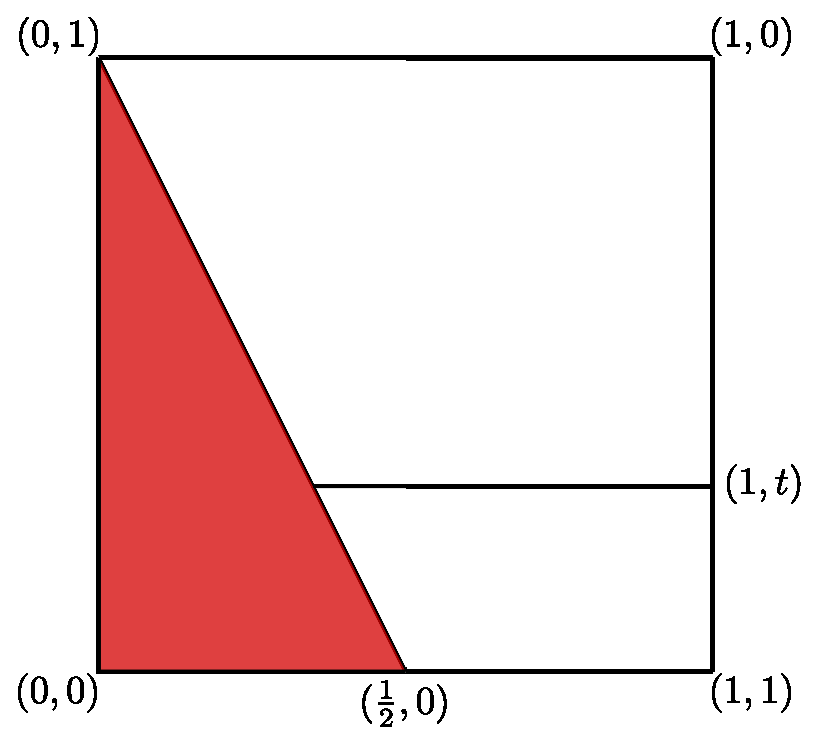
\includegraphics[scale=0.5]{Figures/Chapter4/path_identity.eps}
        \caption{}
        \label{fig_4.1}
    \end{figure}
    of $I \times I$ together with the line joining the points  $(0,1)$ and
    $(\frac{1}{2},0)$. This line has equation $2s=t-1$s. Now, define
    $\theta_t:[\frac{1-t}{2},1] \xrightarrow{} [0,1]$ to be the affine map:
    \begin{equation*}
        \theta_t(s)=\frac{s-\frac{1-t}{2}}{1-\frac{1-t}{2}}
    \end{equation*}
    Define the map $H:I \times I \xrightarrow{} I$ by:
    \begin{equation*}
       H(s,t)=\begin{cases}
                p, & \text{ if } 2s \leq 1-t    \\
                f(\theta_t(s)), & \text{ if } 2s \geq 1-t   \\
            \end{cases}
    \end{equation*}
    By the pasting lemma, $H$ is continuous. Moreover,  $H(0,t)=p=\alpha(f)=i_p
    \ast f$, and $H(1,t)=f(\theta_t(1))=f(t)$. Lastly, $\partial{I}$ is fixed on
    $H$, so we have $i_p \ast f \simeq f \rel{\partial{I}}$. By similar
    reasoning, we also get $f \ast i_q \simeq f \rel{\partial{I}}$.

    Now, conisder the space of figure \ref{4.2}
    \begin{figure}[h]
        \centering
        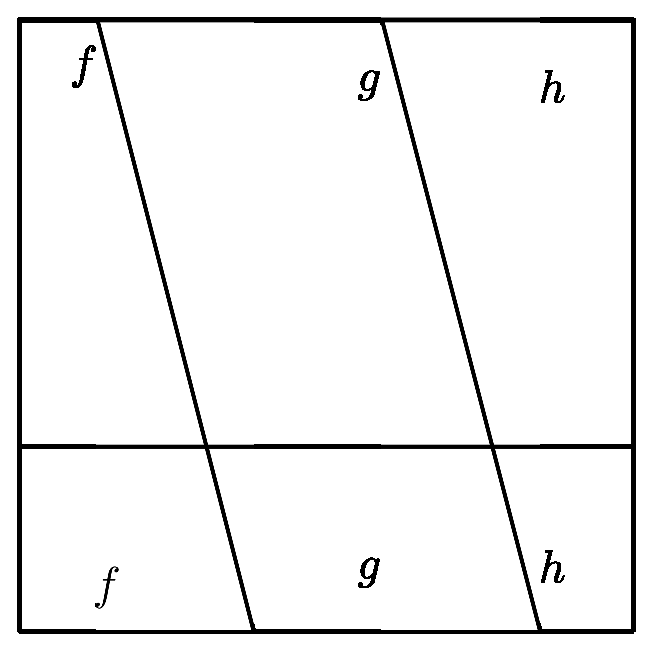
\includegraphics[scale=0.5]{Figures/Chapter4/path_associativity.eps}
        \caption{}
        \label{fig_4.2}
    \end{figure}
    on $I \times I$ togehter with slanted lines. Construct a continuous map
    defined by the affine map from $[0,\frac{1}{2}]$ to $[0,\frac{2-t}{4}]$. It
    follows that $f \ast (g \ast h) \simeq (f \ast g) \ast h \rel{\partial{I}}$.

    Finally, subdivied $I \times I$, again, as in figure \ref{4.3} and define
    the map $H:I \times I \xrightarrow{} X$ by
    \begin{equation*}
       H(s,t)=\begin{cases}
           f(2(s(1-t))), & \text{ if } 0 \leq s \leq \frac{1}{2}    \\
           f(2(1-s)(1-t)), & \text{ if } \frac{1}{2} \leq s \leq 1  \\
            \end{cases}
    \end{equation*}
    This map is continuous by the pasting lemma with $H(0,t)=f \ast \inv{f}$,
    and $H(1,t)=i_q(t)$. Therefore $f \ast \inv{f} \simeq i_p
    \rel{\partial{I}}$. Again by similar reasoning, we get $\inv{f} \ast f
    \simeq i_q \rel{\partial{I}}$.
\end{proof}

\begin{definition}
    Let $X$ be a topological space and  $x_0 \in X$. The \textbf{fundamental
    group} of $X$ with \textbf{basepoint} $x_0$ is the collection of all path
    classes on $X$ which are closed at $x_0$. We denote it $\pi_1(X,x_0)$.
\end{definition}

\begin{theorem}\label{4.1.5}
    The fundamental group of a topoligical space is a group under path
    multiplication for every basepoint in the space.
\end{theorem}
